\documentclass[12pt, letterpaper]{ctexart}

\usepackage[margin=1in]{geometry}
\usepackage{setspace}
\usepackage{graphicx}
\usepackage{booktabs}
\usepackage{array}
\usepackage{siunitx}
\usepackage{hyperref}
\usepackage{amsmath}
\usepackage{caption}
\usepackage{float}
\usepackage{fontspec}

\setmainfont{Times New Roman}
\setCJKmainfont{Songti SC}
\singlespacing
\sisetup{group-separator = {,}, group-minimum-digits = 4}

\hypersetup{
  colorlinks=true,
  linkcolor=black,
  citecolor=black,
  urlcolor=blue
}

\title{第二部分 Case III：界定供款计划与强积金退休规划}
\author{AMA1D03 养老金数学导论}
\date{}

\begin{document}

\begin{titlepage}
  \centering
  \vspace*{2cm}
  {\LARGE\bfseries 第二部分 Case III：\\[0.4em]
  界定供款计划与强积金退休规划\par}
  \vspace{1.5cm}
  {\large AMA1D03 养老金数学导论\par}
  \vfill
  {\large \today\par}
\end{titlepage}
\setcounter{page}{1}

\section*{(a) 界定供款计划的描述及其在养老金体系中的应用}

\subsection*{1. 界定供款（DC）与界定福利（DB）}

在\textbf{界定供款（Defined Contribution, DC）}计划中，\textbf{供款端确定、待遇端不确定}。雇主和/或雇员向个人账户缴付规定金额，终值取决于累计供款、投资回报及费用。投资和长寿风险主要由成员承担。

相比之下，\textbf{界定福利（Defined Benefit, DB）}计划\textbf{待遇端确定、供款端不确定}，主办者依精算假设厘定供款水平，并承担大部分投资与长寿风险。香港的职业退休计划（ORSO）可同时存在 DC 型与 DB 型，与强制性强积金共同构成第二支柱。

香港强积金（MPF）制度于\textbf{2000年12月1日}推出，属于强制性 DC 计划，构成香港退休保障框架的\textbf{第二支柱}：
\begin{itemize}
  \item \textbf{第一支柱：}定额、经审查的现金福利——综援（CSSA，最后安全网）、长者生活津贴（OALA，面向中低收入长者）、高龄津贴（OAA，普惠性较强但金额较低）
  \item \textbf{第二支柱：}强积金强制及自愿供款（以及适用的 ORSO）
  \item \textbf{第三支柱：}个人储蓄、保险及家庭支持
\end{itemize}

香港\textbf{没有任何与收入挂钩的公共养老金}，第一支柱均为定额福利，因此强积金是中产群体退休收入的核心基础——这是香港与加拿大 CPP、美国 Social Security 等体系的本质区别。

\subsection*{2. 强积金计划类型}

根据积金局（MPFA）分类，强积金计划主要分为三类：

\begin{table}[H]
  \centering
  \caption{强积金计划类型}
  \begin{tabular}{@{}p{3.2cm}p{9.8cm}@{}}
    \toprule
    计划类型 & 说明 \\
    \midrule
    集成信托计划 & 可供参与雇主的雇员及自雇人士参加 \\
    雇主营办计划 & 仅供单一雇主的雇员参加 \\
    行业计划 & 供特定行业雇员参加（如饮食业、建造业） \\
    \bottomrule
  \end{tabular}
\end{table}

每名雇员在计划内拥有个人账户。转换工作时，累计权益可转移至新雇主的计划或保留在个人账户中。

\subsection*{3. 强制供款与自愿供款}

\textbf{强制供款（MC）：}
\begin{itemize}
  \item 雇员与雇主各供款\textbf{有关入息的 5\%}
  \item 有关入息设有下限（每月 HK\$7,100）及上限（每月 HK\$30,000）
  \item 月薪低于 HK\$7,100 时，雇员无需强制供款，但雇主仍须按 HK\$7,100 基数的 5\% 供款
  \item 各方最高强制供款额：每月 HK\$1,500
\end{itemize}

\textbf{自愿供款：}
\begin{itemize}
  \item \textbf{计划内自愿供款（VC）：}在强积金计划内额外供款，无薪俸税扣除，提取规则与强制供款一致
  \item \textbf{可扣税自愿供款（TVC）：}独立个人账户，每年最多\textbf{HK\$60,000}可在薪俸税中扣除，提取条件较灵活
\end{itemize}

在 Case III 中，Peter 与 Mary 各供款 HK\$1,000（月薪 HK\$20,000 的 5\%），雇主等额配对，每月总供款为\textbf{HK\$2,000}。

\subsection*{4. 福利、提取与退休年龄}

成员一般可在\textbf{65岁}提取累计权益。其他提取条件包括：永久离港、完全丧失行为能力、罹患末期疾病、60岁停止受雇后提前退休、\textbf{小额结余提取}（累计权益不超过 HK\$5,000）及\textbf{身故权益}给付指定受益人。

提取时，成员可选择一次性提取，或通过强积金平台将部分余额转换为年金。年金的核心功能是\textbf{对冲长寿风险}——这是 DC 模式在成员寿命超过账户余额时的主要短板。

\subsection*{5. 投资选择、回报与费用}

强积金提供多种基金类型：香港、中国、亚洲及全球股票基金；混合资产；债券及保证基金；以及指数基金（如追踪恒生指数基金的 Tracker Fund）。

成员须承担\textbf{投资风险}。基金经理收取管理费（通常每年 0.5\%--2\%），长期会侵蚀净回报。Case III 中，Peter 投资于全球基金，Mary 投资于香港基金，说明在相同供款结构下，资产配置对长期结果的影响。

\subsection*{6. 税务处理与制度角色}

强制强积金供款在法定限额内可获税务豁免。TVC 为希望弥补退休收入缺口的成员提供额外税务优惠。学术及业界研究一致表明，单靠强制供款\textbf{不足以}维持退休前的生活水平，成员须以自愿储蓄及（如符合资格）政府现金福利作补充。

\section*{(b) 界定供款计划的比较与分析——Peter 与 Mary 案例}

\subsection*{1. 模型设定}

本文使用 Python 模型（\texttt{case3/main.py}）模拟自 2000 年 12 月起至各成员年满 65 岁止的按月强积金累积过程。主要假设见表~\ref{tab:assumptions}。

\textbf{假设说明与局限性：}
\begin{itemize}
  \item \textbf{工资增长 = CPI} 等价于\textbf{实际工资零增长}，是较强简化。现实中职业生涯存在实际工资增长，会扩大最终工资分母、进一步降低替代率。
  \item \textbf{收益率：}采用历史月度回报至最新数据，之后拼接\textbf{每年 4\% 名义}未来回报（与积金局长期规划假设一致）。这并非全程历史回测；2000--2025 年全球基金跑赢港股反映特定区间，存在\textbf{后视镜偏差}。
  \item \textbf{4\% 提款法则：}退休首年收入 = 余额的 4\%，隐含后续随通胀调整。该法则针对美国 30 年退休期校准；香港人均预期寿命超 85 岁，固定提取率存在\textbf{长寿耗尽风险}。
  \item \textbf{费率：}1\%/年为强积金中位水平（指数基金可低于 0.5\%；主动股票基金常达 1.2\%--1.8\%），长期复利拖累显著。
\end{itemize}

\begin{table}[H]
  \centering
  \caption{主要建模假设}
  \label{tab:assumptions}
  \small
  \begin{tabular}{@{}lll@{}}
    \toprule
    参数 & 数值 & 说明 \\
    \midrule
    起始日期 & 2000年12月1日 & 强积金推出 \\
    退休年龄 & 65岁 & 正常退休年龄 \\
    初始月薪 & HK\$20,000 & Case III \\
    每月强制供款（雇员+雇主） & HK\$2,000 & 5\% + 5\% \\
    工资增长 & 香港综合消费物价指数 & 实际工资零增长 \\
    香港基金代理 & 恒生指数（\texttt{\^{}HSI}） & 追踪基金追踪恒生指数 \\
    全球基金代理 & 拼接 \texttt{\^{}GSPC}/\texttt{EFA}/\texttt{ACWI} & 2000年12月起完整历史 \\
    未来回报假设 & 每年 4\%（名义） & 最新数据之后 \\
    基金费用率 & 每年 1\% & 强积金中位假设 \\
    退休收入 & 4\% 提款法则 & 首年提取 = 余额的 4\% \\
    \bottomrule
  \end{tabular}
\end{table}

\begin{table}[H]
  \centering
  \caption{Case III 参与者设定}
  \label{tab:participants}
  \begin{tabular}{@{}lcc@{}}
    \toprule
    & Peter & Mary \\
    \midrule
    起始年龄（2000年12月） & 20 & 40 \\
    退休年龄 & 65 & 65 \\
    供款年期 & 45年 & 25年 \\
    退休年份 & 2045 & 2025 \\
    指定基金 & 全球基金（拼接） & 香港基金（\texttt{\^{}HSI}） \\
    \bottomrule
  \end{tabular}
\end{table}

\subsection*{2. 基准情景结果}

\begin{table}[H]
  \centering
  \caption{基准模拟结果}
  \label{tab:baseline}
  \small
  \begin{tabular}{@{}lrr@{}}
    \toprule
    指标 & Peter（全球基金） & Mary（香港基金） \\
    \midrule
    供款年数 & 45.1 & 25.1 \\
    累计供款（HK\$） & 1,443,931 & 723,931 \\
    投资收益（HK\$） & 3,552,431 & 126,930 \\
    退休时强积金余额（HK\$） & \textbf{4,996,362} & \textbf{850,862} \\
    退休前年薪（HK\$） & 555,156 & 374,107 \\
    年退休收入（HK\$） & 199,854 & 34,034 \\
    月退休收入（HK\$） & 16,655 & 2,836 \\
    替代率 & \textbf{36.0\%} & \textbf{9.1\%} \\
    \bottomrule
  \end{tabular}
\end{table}

图~\ref{fig:balance} 显示，Peter 的余额在 45 年内大幅上升，而 Mary 在 25 年内的增长较慢，最终余额约为 Peter 的六分之一。Peter 的投资收益（HK\$355万）远超累计供款（HK\$144万），充分体现了 DC 制度下长期复利的威力。

采用恒生指数完整历史数据后，Mary 的供款期覆盖了 2000 年后港股大幅波动（包括 2008 年金融危机），其最终余额较此前不完整数据估计更低，结论更为保守。

\begin{figure}[H]
  \centering
  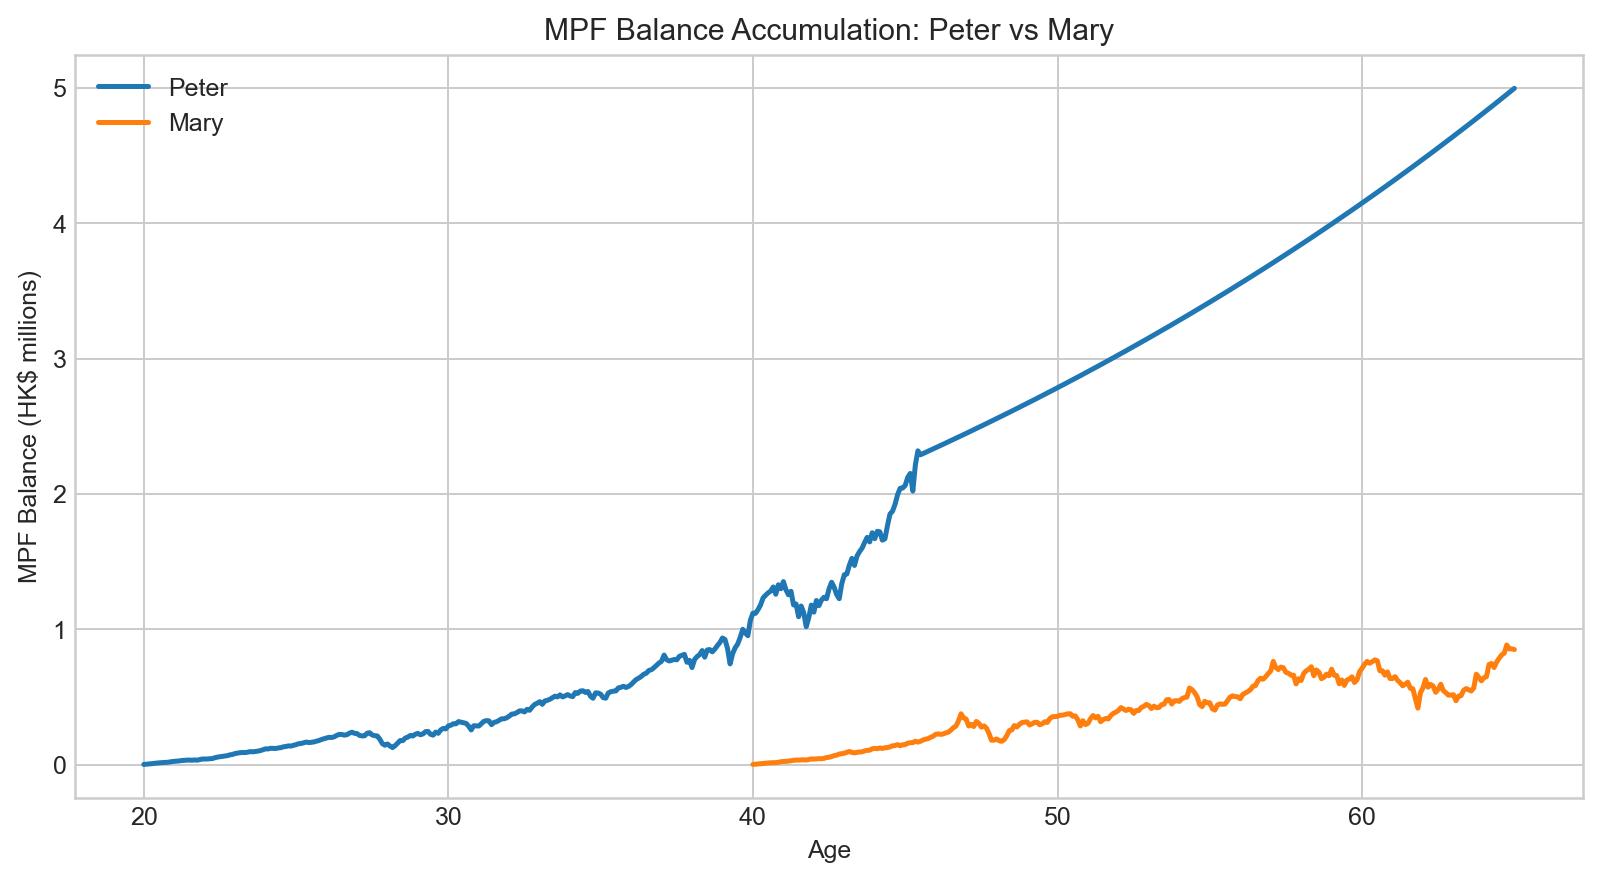
\includegraphics[width=0.92\textwidth]{../output/fig1_balance_over_age.png}
  \caption{强积金余额累积：Peter 与 Mary 比较}
  \label{fig:balance}
\end{figure}

\subsection*{3. 优势与劣势}

\textbf{优势：}
\begin{enumerate}
  \item \textbf{产权清晰、可携带：}个人账户适配香港高流动性劳动力市场；无 DB 计划的雇主信用风险。
  \item \textbf{雇主配对供款：}雇主 5\% 供款在不增加雇员成本的情况下使储蓄翻倍。
  \item \textbf{投资选择：}成员可按风险偏好选择基金。
  \item \textbf{税务优惠：}TVC 每年最多 HK\$60,000 可扣税。
  \item \textbf{复利效应：}尽早供款受惠于数十年复利（「72 法则」：年化 4\% 约 18 年翻倍；45 年约 6 倍复利，25 年仅约 2.7 倍）。
\end{enumerate}

\textbf{劣势：}
\begin{enumerate}
  \item \textbf{投资与序列风险：}成员承担全部下跌风险；退休前市场暴跌会大幅侵蚀终值。
  \item \textbf{缺乏风险共担：}与 DB 不同，无长寿或投资短缺的跨期补贴。
  \item \textbf{替代率偏低：}即使 Peter 的强制供款替代率亦仅 36\%，低于通常建议的 60--70\%。
  \item \textbf{费用与行为侵蚀：}管理费产生负面复利；非理性换基金进一步降低净回报。
  \item \textbf{迟供款惩罚：}Mary 9.1\% 的替代率表明，40岁才开始供款无法仅靠选基金弥补。
\end{enumerate}

\subsection*{4. 起始年龄与基金选择孰轻孰重}

表~\ref{tab:age} 列示不同起始年龄的替代率；表~\ref{tab:fundswap} 列示互换基金后的敏感性结果。

\begin{table}[H]
  \centering
  \caption{不同起始年龄与基金的替代率}
  \label{tab:age}
  \small
  \begin{tabular}{@{}ccrr@{}}
    \toprule
    起始年龄 & 基金 & 最终余额（HK\$） & 替代率 \\
    \midrule
    20 & 全球 & 4,996,362 & 36.0\% \\
    20 & 香港 & 2,427,886 & 17.5\% \\
    30 & 全球 & 3,417,078 & 30.0\% \\
    30 & 香港 & 1,500,213 & 13.2\% \\
    40 & 全球 & 2,063,587 & 22.1\% \\
    40 & 香港 & 850,862 & 9.1\% \\
    50 & 全球 & 520,922 & 6.9\% \\
    50 & 香港 & 457,617 & 6.0\% \\
    \bottomrule
  \end{tabular}
\end{table}

\begin{table}[H]
  \centering
  \caption{基金互换敏感性分析}
  \label{tab:fundswap}
  \begin{tabular}{@{}lccc@{}}
    \toprule
    姓名 & 指定基金替代率 & 互换后替代率 & 变化（百分点） \\
    \midrule
    Peter（20岁） & 36.0\% & 17.5\% & $-18.5$ \\
    Mary（40岁） & 9.1\% & 22.1\% & $+13.0$ \\
    \bottomrule
  \end{tabular}
\end{table}

\textbf{主要发现：}在相同基金下比较起始年龄，20岁与40岁（全球/香港基金）的替代率相差\textbf{27个百分点}（36\% 对 9.1\%）。Peter 在20岁时即使选择表现较差的香港基金（17.5\%），最终余额仍远高于 Mary。\textbf{供款年期比基金选择更为重要}——终值对时间的敏感度为指数级，对收益率仅为幂次级。

\begin{figure}[H]
  \centering
  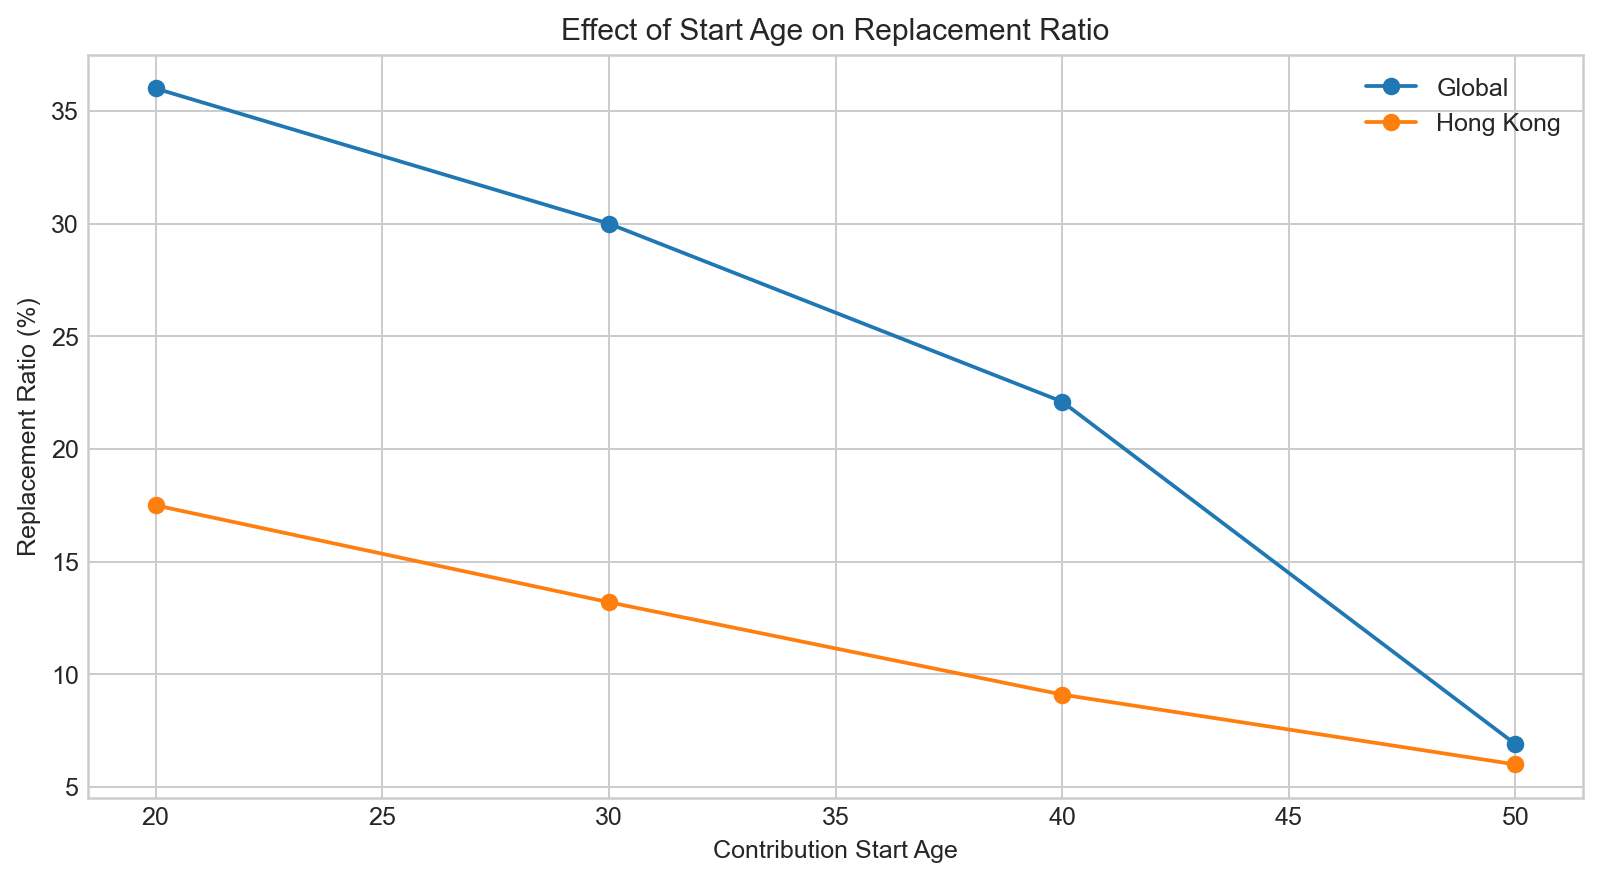
\includegraphics[width=0.92\textwidth]{../output/fig3_start_age_sensitivity.png}
  \caption{起始年龄对替代率的影响}
  \label{fig:age}
\end{figure}

\subsection*{5. 生活开支、通胀与额外供款}

财务规划通常以\textbf{60--70\%替代率}为目标。按表~\ref{tab:baseline}最终月薪计算（$60\% \times$ 最终月薪 $-$ 强积金月收入）：Peter 缺口约 HK\$11,103；Mary 缺口约 HK\$15,870。

工资及强制供款随消费物价指数调整，但退休收入的实际购买力取决于投资回报能否跑赢通胀。45 年内 1\% 的费用差异可显著降低最终余额（敏感性测算：Peter 在 1\% 费率下余额 HK\$499 万，1.5\% 费率下降至约 HK\$432 万）。

\begin{table}[H]
  \centering
  \caption{达到目标替代率所需的 TVC}
  \label{tab:tvc}
  \begin{tabular}{@{}lccc@{}}
    \toprule
    成员 & 当前替代率 & 目标替代率 & 每月额外 TVC（HK\$） \\
    \midrule
    Peter & 36.0\% & 60\% & 1,582 \\
    Peter & 36.0\% & 70\% & 2,242 \\
    Mary & 9.1\% & 60\% & 13,205 \\
    Mary & 9.1\% & 70\% & 15,799 \\
    \bottomrule
  \end{tabular}
\end{table}

\begin{figure}[H]
  \centering
  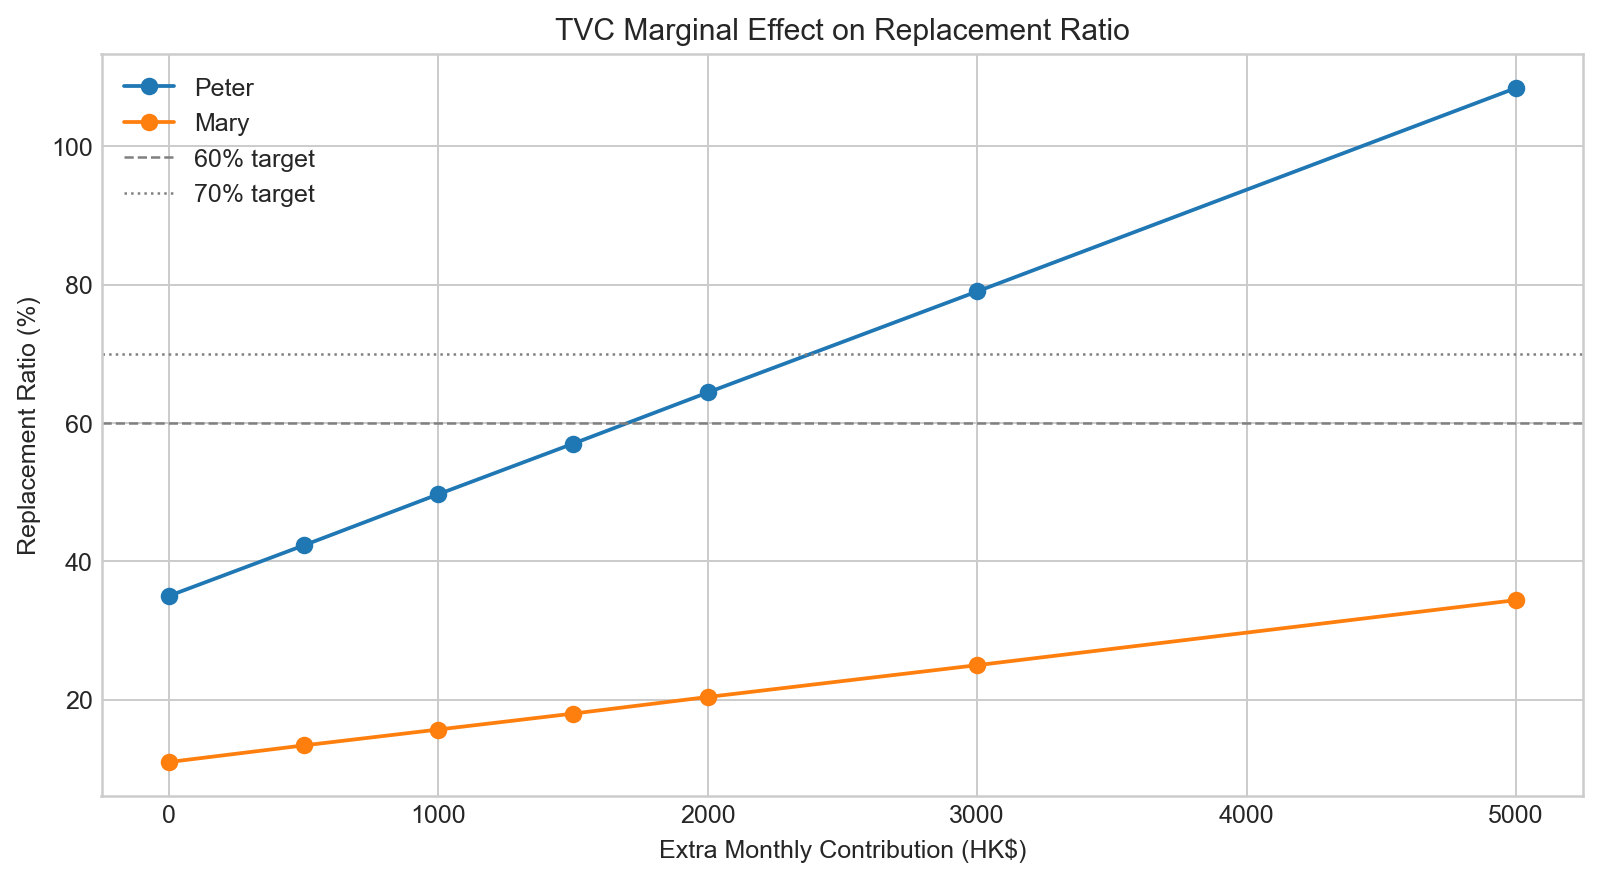
\includegraphics[width=0.92\textwidth]{../output/fig4_tvc_marginal_effect.png}
  \caption{TVC 对替代率的边际效应}
  \label{fig:tvc}
\end{figure}

Mary 迫切需要大量 TVC 或其他收入来源。Peter 要达到 60\% 替代率，每月仍需约 HK\$1,600 额外供款，可在 TVC 扣税上限内实现（每年 HK\$60,000 $\approx$ 每月 HK\$5,000）。Mary 所需每月 TVC 约 HK\$13,205，远超免税额度——仅前 HK\$5,000/月可扣税，余额须通过不可扣税 VC 或第三支柱储蓄补足。

\section*{(c) 结合社会保障制度支持 DC 计划下的退休生活}

\subsection*{1. 香港三支柱框架}

与加拿大 CPP 或美国 Social Security 不同，香港\textbf{没有}全民、与收入挂钩的公共养老金。政府支持以资产审查为主，呈\textbf{分层兜底}结构：
\begin{itemize}
  \item \textbf{第一支柱}覆盖低资产、低收入长者（综援审查最严；OALA 经资产/收入审查；OAA 较普惠但金额较低）
  \item \textbf{第二支柱}（强积金）为所有就业人士的强制基础积累
  \item \textbf{第三支柱}是维持退休前生活水平的主要杠杆
\end{itemize}

对 Peter、Mary 这类中产雇员，当强积金余额计入资产审查时，第一支柱福利\textbf{基本无法享受}——退休收入须依靠强积金与自愿储蓄，而非三支柱简单叠加。

\subsection*{2. 长者生活津贴（OALA）}

年满65岁的合资格香港居民可领取普通 OALA（每月 HK\$2,065）或高额 OALA（每月 HK\$4,185）（2025/26 年度），须通过收入及资产审查。单身人士两类 OALA 的资产上限约为 HK\$401,000。\textbf{尚未提取的强积金权益计入资产}，形成\textbf{挤出效应}：DC 积累越多，越难享受第一支柱福利——二者并非简单叠加。

\subsection*{3. 综合退休收入}

表~\ref{tab:income}列示\textbf{实际}资格审查结果。Peter（强积金余额 HK\$499 万）与 Mary（HK\$85.1 万）均远超资产上限，计入强积金后\textbf{均不符合 OALA 资格}。表~\ref{tab:income_hyp}仅作假设性对照（若资产低于上限）。

\begin{table}[H]
  \centering
  \caption{经 OALA 资产审查后的退休收入（强积金计入资产）}
  \label{tab:income}
  \small
  \begin{tabular}{@{}l r r r r r@{}}
    \toprule
    成员 & 强积金余额 & 资产上限 & 强积金收入 & OALA & 综合替代率 \\
    \midrule
    Peter & 4,996,362 & 401,000 & 16,655 & 0 & 36.0\% \\
    Mary & 850,862 & 401,000 & 2,836 & 0 & 9.1\% \\
    \bottomrule
  \end{tabular}
\end{table}

\begin{table}[H]
  \centering
  \caption{假设性 OALA 情景（若强积金不计入资产——不适用于 Case III）}
  \label{tab:income_hyp}
  \small
  \begin{tabular}{@{}l l r r r r@{}}
    \toprule
    成员 & 情景 & 强积金 & OALA & 合计 & 综合替代率 \\
    \midrule
    Peter & 普通 OALA & 16,655 & 2,065 & 18,720 & 40.5\% \\
    Peter & 高额 OALA & 16,655 & 4,185 & 20,840 & 45.0\% \\
    Mary & 普通 OALA & 2,836 & 2,065 & 4,901 & 15.7\% \\
    Mary & 高额 OALA & 2,836 & 4,185 & 7,021 & 22.5\% \\
    \bottomrule
  \end{tabular}
\end{table}

\begin{figure}[H]
  \centering
  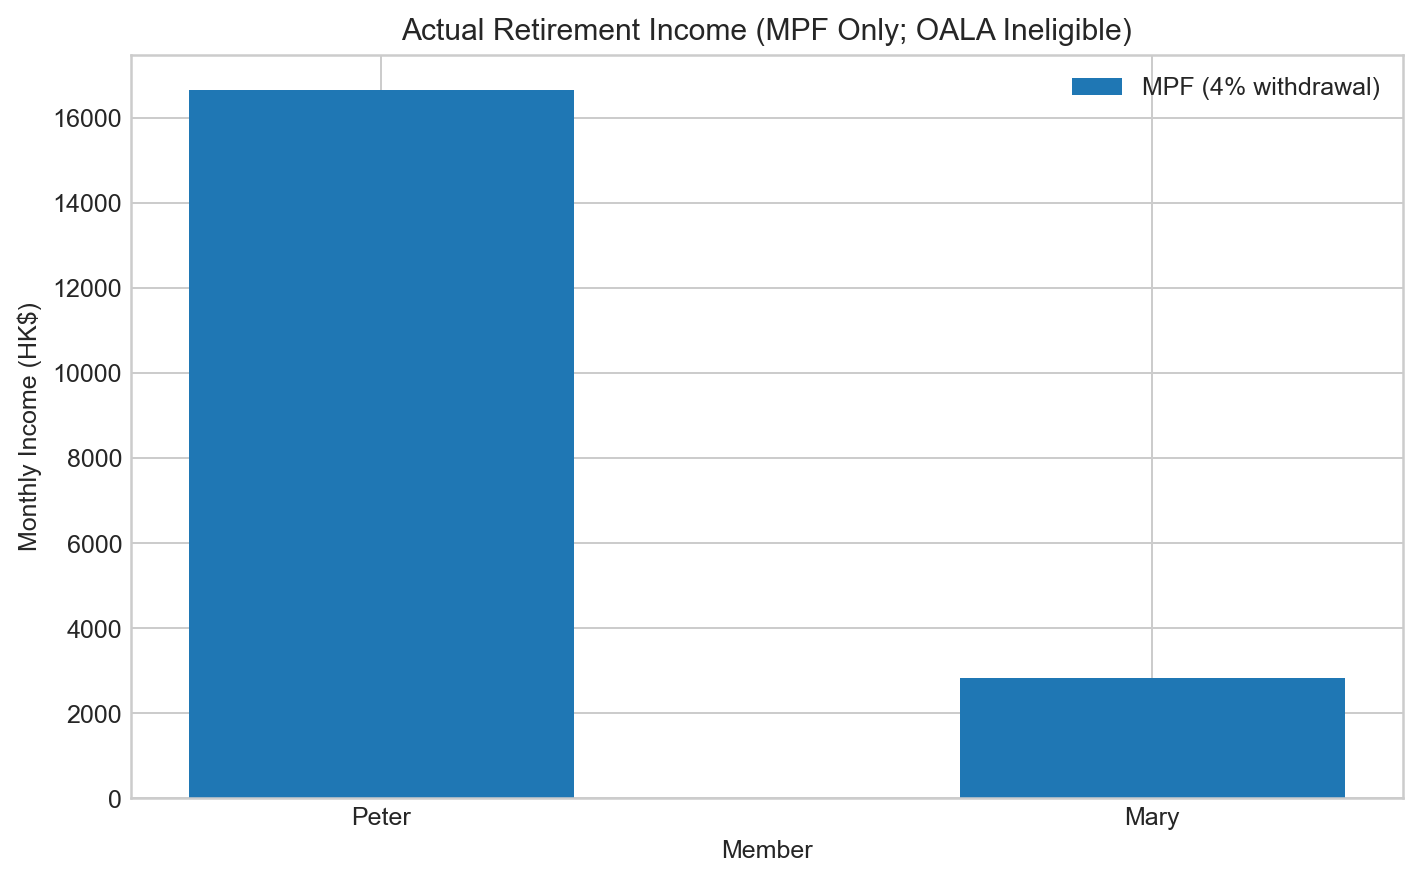
\includegraphics[width=0.78\textwidth]{../output/fig2_income_breakdown.png}
  \caption{实际退休收入（仅强积金；资产审查下不符合 OALA）}
  \label{fig:income}
\end{figure}

\subsection*{4. 策略示例}

\textbf{Peter（2045年退休）：}
\begin{itemize}
  \item 强积金提供良好基础（替代率 36\%），但预期强积金资产下\textbf{不符合 OALA 资格}。
  \item 每月增加约 HK\$1,600 TVC，可使强积金单独达到 60\% 替代率（在 TVC 扣税上限内）。
  \item 采用\textbf{生命周期配置}：年轻时高权益比例，55 岁后逐步增配债券/保本基金，降低退休前序列风险——而非 45 年全程持有全球股票。
  \item 将部分强积金余额年金化，构建终身最低收入底仓，对冲长寿风险。
\end{itemize}

\textbf{Mary（2025年退休）：}
\begin{itemize}
  \item 单靠强制强积金严重不足（替代率 9.1\%）；强积金余额 HK\$85.1 万 $>$ 上限，\textbf{不符合 OALA}。
  \item 延迟退休至 70 岁仅将替代率小幅提升至 10.9\%——多供款几年无法弥补 20 年错过的复利。
  \item 所需额外储蓄远超 TVC 免税额度，须结合不可扣税 VC、第三支柱储蓄及可能的兼职收入。
  \item 在账户规模有限时，年金化与延迟提取仍可改善收入保障。
\end{itemize}

Mary 的现实方案——强积金（HK\$2,836）+ 第三支柱储蓄或兼职（如每月 HK\$5,000）——约 HK\$7,836/月，仍低于 60\% 目标 HK\$18,706。即使假设性高额 OALA 情景（表~\ref{tab:income_hyp}）亦仅达 22.5\%。

\begin{table}[H]
  \centering
  \caption{Mary：延迟退休敏感性}
  \label{tab:delay}
  \begin{tabular}{@{}lrrr@{}}
    \toprule
    退休年龄 & 供款年数 & 强积金余额（HK\$） & 替代率 \\
    \midrule
    65 & 25.1 & 850,862 & 9.1\% \\
    67 & 27.1 & 930,635 & 9.6\% \\
    70 & 30.1 & 1,128,770 & 10.9\% \\
    \bottomrule
  \end{tabular}
\end{table}

\subsection*{5. 关于额外供款的结论}

\begin{table}[H]
  \centering
  \caption{建议摘要}
  \label{tab:conclusion}
  \begin{tabular}{@{}lcc@{}}
    \toprule
    问题 & Peter & Mary \\
    \midrule
    强制强积金是否足够？ & 否（36\%） & 否（9.1\%） \\
    是否应增加 TVC？ & 是，适度 & 是，迫切 \\
    社会保障能否填补缺口？ & 否（资产审查） & 否（资产审查） \\
    \bottomrule
  \end{tabular}
\end{table}

香港的 DC 制度将退休责任转移至个人。像 Peter 一样尽早、持续供款是最有效的杠杆。社会保障（OALA）为\textbf{低资产}退休人员提供安全网，但对有可观强积金积累的中产群体存在挤出效应。\textbf{Peter 与 Mary 均应增加额外供款，其中 Mary 的紧迫性及所需金额远高于 Peter。}

\subsection*{6. 核心结论}

\begin{enumerate}
  \item 单靠强制强积金无法维持退休前生活水平，自愿供款是必然选择。
  \item \textbf{供款起始时间}是 DC 计划下退休收入的核心决定因素——时间复利效应远大于基金选择。
  \item 香港第一支柱仅能发挥底线兜底作用，无法填补中产群体的退休缺口。
  \item 完整退休规划须结合「强制 + 自愿强积金、第三支柱储蓄、生命周期降风险、部分年金化」。
\end{enumerate}

\section*{主要公式}

随 CPI 增长的供款累积终值（按月模拟）：
\begin{equation}
  FV = \sum_{t=1}^{n} PMT_0 (1+g)^{t-1} \prod_{k=t+1}^{n}(1+r_k)
\end{equation}
其中 $PMT_0$ 为初始月度供款，$g$ 为供款年增长率（CPI），$r_k$ 为第 $k$ 期净回报率，$n$ 为供款总期数。

当 $r$ 与 $g$ 为常数且 $r \neq g$ 时，增长年金闭式解为：
\begin{equation}
  FV = PMT_0 (1+r) \cdot \frac{(1+r)^n - (1+g)^n}{r - g}
\end{equation}

采用 4\% 提款率的替代率：
\begin{equation}
  RR = \frac{FV \times 0.04}{Salary_{final}}
\end{equation}

达到目标替代率 $\rho^*$ 所需月度 TVC：对 $PMT_{TVC}$ 求解
\begin{equation}
  \rho^* = \frac{0.04 \times FV(PMT_0, g, r, n) + 0.04 \times FV(PMT_{TVC}, g, r, n')}{Salary_{final}}
\end{equation}
其中 $n'$ 为额外供款期数（本案例为完整供款年期）。表~\ref{tab:tvc} 数值由模拟模型二分搜索求得。

达到 60\% 目标的月度收入缺口：
\begin{equation}
  Gap_{monthly} = 0.60 \times \frac{Salary_{final}}{12} - \frac{FV_{MPF} \times 0.04}{12}
\end{equation}

\begin{thebibliography}{9}
  \bibitem{mpfa} 强制性公积金计划管理局，《强积金基金表现平台》，\url{https://mfp.mpfa.org.hk/}。
  \bibitem{swd} 社会福利署，《长者生活津贴》，\url{https://www.swd.gov.hk/oala/}。
  \bibitem{csd} 政府统计处，《综合消费物价指数》。
  \bibitem{ira} Investopedia, \textit{Individual Retirement Account (IRA)}, \url{https://www.investopedia.com/terms/i/ira.asp}.
\end{thebibliography}

\appendix
\section*{附录：模拟结果复现说明}

所有数值结果由 \texttt{case3/} 目录下的 Python 程序生成。复现表格与图表请执行：
\begin{verbatim}
cd case3
python3 main.py
python3 src/validate.py
\end{verbatim}

输出文件存放于 \texttt{case3/output/}，假设说明见 \texttt{case3/data/assumptions.md}。

\end{document}
